% Day 1 - Waves: hands-on background (FoamWaveTank training)
% Build:  pdflatex Day1_Waves_HandsOn.tex  (run twice)
\documentclass[aspectratio=169,10pt]{beamer}

\usepackage[T1]{fontenc}
\usepackage{lmodern}
\usepackage{amsmath}
\usepackage{booktabs}
\usepackage{tabularx}
\usepackage{array}
\newcolumntype{L}{>{\raggedright\arraybackslash}X}
\newcolumntype{P}[1]{>{\raggedright\arraybackslash}p{#1}}
\usepackage{listings}
\usepackage{tikz}
\usepackage{pgfplots}
\pgfplotsset{compat=1.17}
\usetikzlibrary{arrows.meta,positioning,calc,shapes.geometric,decorations.pathmorphing}

% ---------------------------------------------------------------- colours
\definecolor{deep}{HTML}{0B3C49}
\definecolor{sea}{HTML}{1A7F8E}
\definecolor{foam}{HTML}{EAF4F4}
\definecolor{sand}{HTML}{F2A541}
\definecolor{coral}{HTML}{C8414F}
\definecolor{ink}{HTML}{1F2A30}
\definecolor{mute}{HTML}{5C6B73}
\definecolor{codebg}{HTML}{F3F6F7}

% ---------------------------------------------------------------- beamer look
\usetheme{default}
\setbeamertemplate{navigation symbols}{}
\setbeamercolor{normal text}{fg=ink}
\setbeamercolor{frametitle}{fg=deep}
\setbeamercolor{structure}{fg=sea}
\setbeamercolor{alerted text}{fg=coral}
\setbeamerfont{frametitle}{size=\Large,series=\bfseries}
\setbeamertemplate{itemize items}{\color{sea}\raisebox{0.15ex}{\tiny$\blacksquare$}}
\setbeamertemplate{itemize subitem}{\color{mute}--}
\setbeamertemplate{enumerate items}[default]
\setbeamertemplate{frametitle}{\vspace*{0.3em}\insertframetitle\par\vspace*{-0.2em}}
\setbeamertemplate{footline}{%
  \hbox{\hspace*{1em}\color{mute}\tiny FoamWaveTank training \,$\cdot$\, Day 1: Waves
  \hfill\insertframenumber\hspace*{1em}}\vspace*{0.6em}}

\newcommand{\sectionframe}[2]{%
  {\setbeamercolor{background canvas}{bg=deep}
   \setbeamertemplate{footline}{}
   \begin{frame}[plain]
     \vfill
     {\color{sand}\large\bfseries #1}\par\vspace{0.4em}
     {\color{white}\huge\bfseries #2}
     \vfill
   \end{frame}}}

\newcommand{\file}[1]{{\leavevmode\ttfamily\color{deep}#1}}
\newcommand{\key}[1]{{\leavevmode\ttfamily\color{sea}#1}}

% ---------------------------------------------------------------- listings
\lstdefinelanguage{foam}{
  morecomment=[l]{//}, morecomment=[s]{/*}{*/}, morecomment=[l]{\#},
  morestring=[b]",
  morekeywords={waveType,height,period,depth,direction,phi,Tsoft,
    relaxationZone,relaxationScheme,relaxationShape,beachType,relaxType,startX,endX,orientation,
    spectrum,Hs,Tp,gamma,N,phaseMethod,seedForRandomPhase,frequencyAxis,etaMax,focusTime,focusPoint,
    seaLevel,relaxationNames,initializationName,externalForcing,Grid2Grid,Grid2GridCoeffs,
    Grid2GridInputFileName,referencePosition,referenceTheta,referenceTime,
    type,fileType,filePath,interpolationOrder,zMeshType,zMin,zMax,nZMin,nZMax,zMinRatio,zMaxRatio,
    pointDistribution,xValues,yValues,zValues,add,axis,writeControl,writeInterval,
    inletCoeffs,outletCoeffs,U,discretisation,lowerFrequencyCutoff,upperFrequencyCutoff,writeSpectrum}
}
\lstset{
  basicstyle=\ttfamily\scriptsize\color{ink},
  keywordstyle=\color{sea}\bfseries,
  commentstyle=\color{mute}\itshape,
  stringstyle=\color{coral},
  backgroundcolor=\color{codebg},
  frame=none, framesep=0pt, xleftmargin=4pt, xrightmargin=4pt,
  aboveskip=2pt, belowskip=2pt,
  columns=fullflexible, keepspaces=true, showstringspaces=false,
  breaklines=false, tabsize=4, upquote=true
}
\lstdefinestyle{sh}{language=bash, morekeywords={runApplication,python3,cd,cp},
  keywordstyle=\color{sea}\bfseries}

\tikzset{
  box/.style={draw=sea, fill=foam, rounded corners=3pt, thick, align=center,
              font=\scriptsize, inner sep=4pt},
  dbox/.style={draw=deep, fill=deep, text=white, rounded corners=3pt, thick, align=center,
               font=\scriptsize\bfseries, inner sep=4pt},
  arr/.style={-{Stealth[length=2.5mm]}, thick, color=deep},
}

\title{Day 1: Waves in FoamWaveTank}
\subtitle{Hands-on background: wave input, mesh, gauges, solver set-up,\\
          HOS-NWT and the Grid2Grid coupling}
\date{}

\begin{document}

% ======================================================================
{\setbeamercolor{background canvas}{bg=deep}
 \setbeamertemplate{footline}{}
\begin{frame}[plain]
  \vfill
  {\color{sand}\large\bfseries FoamWaveTank training}\par\vspace{0.5em}
  {\color{white}\fontsize{30}{34}\selectfont\bfseries Day 1: Waves}\par\vspace{0.8em}
  {\color{foam}\normalsize Hands-on background: wave input, mesh, gauges, solver set-up,\\
   HOS-NWT and the Grid2Grid coupling}
  \vfill
  
\begin{tikzpicture}
    \draw[sand, very thick, domain=0:14, samples=200]
      plot (\x, {0.25*sin(deg(2*pi*\x/2.8)) + 0.04*sin(deg(4*pi*\x/2.8))});
  \end{tikzpicture}
  \vfill
\end{frame}}

% ======================================================================
\begin{frame}{The day in three parts}
  \centering
  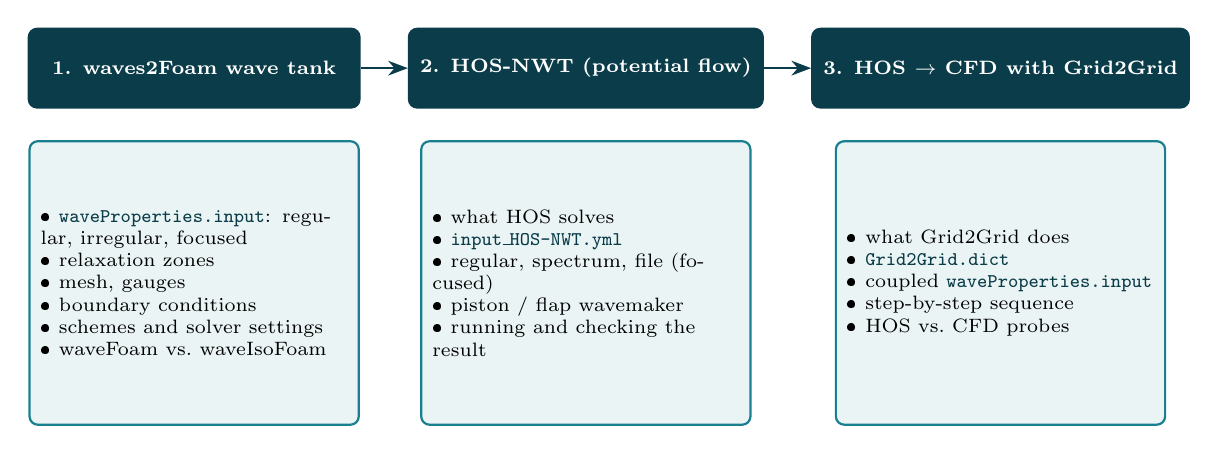
\begin{tikzpicture}[node distance=6mm]
    \node[dbox, minimum width=4.2cm, minimum height=1cm] (a) {1. waves2Foam wave tank};
    \node[dbox, minimum width=4.2cm, minimum height=1cm, right=of a] (b) {2. HOS-NWT (potential flow)};
    \node[dbox, minimum width=4.2cm, minimum height=1cm, right=of b] (c) {3. HOS $\rightarrow$ CFD with Grid2Grid};
    \draw[arr] (a) -- (b); \draw[arr] (b) -- (c);
    \node[box, below=4mm of a, text width=3.9cm, align=left, minimum height=3.6cm, anchor=north] {%
      \textbullet\ \file{waveProperties.input}: regular, irregular, focused\\
      \textbullet\ relaxation zones\\
      \textbullet\ mesh, gauges\\
      \textbullet\ boundary conditions\\
      \textbullet\ schemes and solver settings\\
      \textbullet\ waveFoam vs.\ waveIsoFoam};
    \node[box, below=4mm of b, text width=3.9cm, align=left, minimum height=3.6cm, anchor=north] {%
      \textbullet\ what HOS solves\\
      \textbullet\ \file{input\_HOS-NWT.yml}\\
      \textbullet\ regular, spectrum, file (focused)\\
      \textbullet\ piston / flap wavemaker\\
      \textbullet\ running and checking the result};
    \node[box, below=4mm of c, text width=3.9cm, align=left, minimum height=3.6cm, anchor=north] {%
      \textbullet\ what Grid2Grid does\\
      \textbullet\ \file{Grid2Grid.dict}\\
      \textbullet\ coupled \file{waveProperties.input}\\
      \textbullet\ step-by-step sequence\\
      \textbullet\ HOS vs.\ CFD probes};
  \end{tikzpicture}

  \vspace{3mm}
  {\small Cases: \file{Day1\_Waves/HandsonExercise/\{waveFoam, waveIsoFoam, potentialFlowWaves\}}}
\end{frame}

% ======================================================================
\sectionframe{Part 1}{The waves2Foam numerical wave tank}

% ----------------------------------------------------------------------
\begin{frame}{The 2D wave flume of the Day 1 cases}
  \centering
  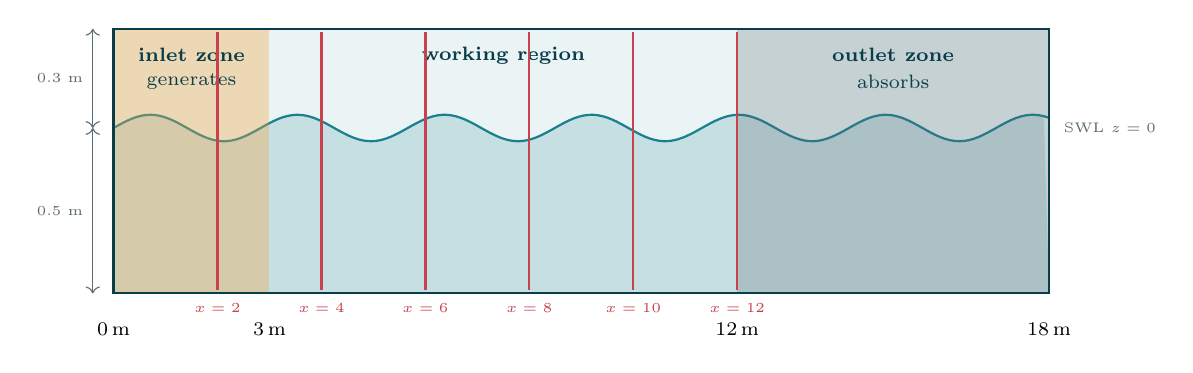
\begin{tikzpicture}[x=0.66cm, y=4.2cm]
    % water and air
    \fill[foam] (0,-0.5) rectangle (18,0.3);
    \fill[sea!25] (0,-0.5) -- (0,0)
      \foreach \x in {0,0.1,...,18} { -- (\x,{0.04*sin(deg(2*pi*\x/2.83))}) } -- (18,-0.5) -- cycle;
    \draw[sea, thick, domain=0:18, samples=200] plot (\x,{0.04*sin(deg(2*pi*\x/2.83))});
    % zones
    \fill[sand, opacity=0.35] (0,-0.5) rectangle (3,0.3);
    \fill[mute, opacity=0.25] (12,-0.5) rectangle (18,0.3);
    \draw[deep, thick] (0,-0.5) rectangle (18,0.3);
    \node[font=\scriptsize\bfseries, deep] at (1.5,0.22) {inlet zone};
    \node[font=\scriptsize, deep] at (1.5,0.14) {generates};
    \node[font=\scriptsize\bfseries, deep] at (15,0.22) {outlet zone};
    \node[font=\scriptsize, deep] at (15,0.14) {absorbs};
    \node[font=\scriptsize\bfseries, deep] at (7.5,0.22) {working region};
    % gauges
    \foreach \x in {2,4,6,8,10,12} {
      \draw[coral, thick] (\x,-0.49) -- (\x,0.29);
      \node[font=\tiny, coral, below] at (\x,-0.5) {$x=\x$};
    }
    % axis
    \foreach \x in {0,3,12,18} \node[font=\scriptsize, below] at (\x,-0.56) {\x\,m};
    \draw[<->, mute] (-0.4,-0.5) -- node[left, font=\tiny] {0.5 m} (-0.4,0);
    \draw[<->, mute] (-0.4,0) -- node[left, font=\tiny] {0.3 m} (-0.4,0.3);
    \node[font=\tiny, mute, right] at (18.1,0) {SWL $z=0$};
  \end{tikzpicture}

  \vspace{2mm}
  \begin{columns}[T]
    \column{0.48\textwidth}\small
    \begin{itemize}
      \item 18 m long, 0.5 m deep, 0.3 m air above
      \item 2D: one cell across, \key{frontBack} is \key{empty}
      \item 6 wave gauges (red), $x$ = 2 \dots 12 m
    \end{itemize}
    \column{0.48\textwidth}\small
    \begin{itemize}
      \item The wave enters through the \textbf{inlet relaxation zone}
      \item The \textbf{outlet zone} (6 m, two wave lengths) removes it
      \item The boundaries themselves are passive
    \end{itemize}
  \end{columns}
\end{frame}

% ----------------------------------------------------------------------
\begin{frame}[fragile]{What \texttt{Allrun} does}
  \centering
  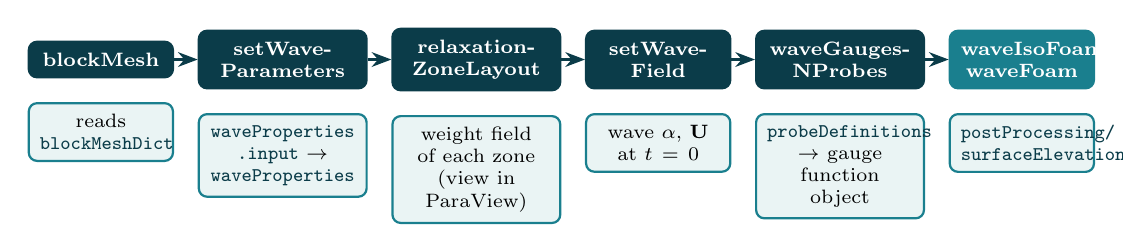
\begin{tikzpicture}[node distance=3mm]
    \node[dbox, text width=1.55cm] (m) {blockMesh};
    \node[dbox, text width=1.85cm, right=of m] (p) {setWave-\\Parameters};
    \node[dbox, text width=1.85cm, right=of p] (r) {relaxation-\\ZoneLayout};
    \node[dbox, text width=1.55cm, right=of r] (f) {setWave-\\Field};
    \node[dbox, text width=1.85cm, right=of f] (g) {waveGauges-\\NProbes};
    \node[dbox, text width=1.55cm, right=of g, fill=sea, draw=sea] (s) {waveIsoFoam\\waveFoam};
    \foreach \a/\b in {m/p,p/r,r/f,f/g,g/s} \draw[arr] (\a) -- (\b);
    \node[box, below=3mm of m, text width=1.55cm] {reads\\\file{blockMeshDict}};
    \node[box, below=3mm of p, text width=1.85cm] {\file{waveProperties\\.input} $\rightarrow$\\\file{waveProperties}};
    \node[box, below=3mm of r, text width=1.85cm] {weight field\\of each zone\\(view in ParaView)};
    \node[box, below=3mm of f, text width=1.55cm] {wave $\alpha$, $\mathbf{U}$\\at $t=0$};
    \node[box, below=3mm of g, text width=1.85cm] {\file{probeDefinitions}\\$\rightarrow$ gauge\\function object};
    \node[box, below=3mm of s, text width=1.55cm] {\file{postProcessing/\\surfaceElevation}};
  \end{tikzpicture}

  \vspace{4mm}
\begin{lstlisting}[style=sh]
runApplication blockMesh;          runApplication checkMesh
runApplication setWaveParameters   # waveProperties.input -> waveProperties
runApplication relaxationZoneLayout
runApplication setWaveField        # alpha, U (and p) of the wave at t = 0
runApplication waveGaugesNProbes   # writes waveGaugesNProbes/surfaceElevation_controlDict
runApplication $(getApplication)   # application in system/controlDict
\end{lstlisting}
  \small Each tool writes \file{log.<tool>}. When a step fails, check its log first.
\end{frame}

% ----------------------------------------------------------------------
\begin{frame}[fragile]{setWaveParameters: from your input to the solver}
  \begin{columns}[T]
    \column{0.47\textwidth}
    \small You give the \textbf{physical wave}, e.g.\ $H$, $T$, $h$.
    \texttt{setWaveParameters} computes the derived quantities and writes them, with your input,
    to \file{constant/waveProperties}:
    \begin{itemize}
      \item $\omega = 2\pi/T$
      \item wave number $k$ from the dispersion relation\\
            $\omega^2 = g\,k\tanh(kh)$
      \item spectra: amplitude, $\omega$, $k$ and phase of each of the $N$ components
      \item focused: phases that put all crests at $(x_f, t_f)$
    \end{itemize}
    \alert{Edit \file{waveProperties.input}, never \file{waveProperties}.} It is overwritten at every run.

    \column{0.5\textwidth}
    \small\textbf{Structure of \file{waveProperties.input}}
\begin{lstlisting}[language=foam]
seaLevel            0.0;      // still water z
relaxationNames     (inlet outlet);
initializationName  inlet;    // t = 0 field

inletCoeffs                   // <name>Coeffs
{
    waveType    ... ;         // wave theory
    ...                       // its parameters
    Tsoft       3;            // ramp-up [s]
    relaxationZone { ... }    // where / how
};

outletCoeffs
{
    waveType    potentialCurrent;
    U           (0 0 0);      // relax to rest
    relaxationZone { ... }
};
\end{lstlisting}
  \end{columns}
\end{frame}

% ----------------------------------------------------------------------
\begin{frame}[fragile]{Regular waves: \texttt{01\_regularWaves}}
  \begin{columns}[T]
    \column{0.5\textwidth}
\begin{lstlisting}[language=foam]
inletCoeffs
{
    waveType    stokesSecond;
    height      0.08;      // H [m]
    period      1.5;       // T [s]
    depth       0.5;       // h [m]
    direction   (1 0 0);   // propagates +x
    phi         0.0;       // phase [rad]
    debug       off;
    Tsoft       3;         // ramp-up [s]

    relaxationZone { ... } // x = 0 .. 3 m
};
\end{lstlisting}
    \column{0.47\textwidth}\small
    \textbf{This wave}
    \begin{itemize}
      \item $L = 2.83$ m, $kh = 1.11$ (intermediate depth)
      \item steepness $H/L \approx 0.028$
      \item Ursell number $HL^2/h^3 \approx 5$: Stokes theory is fine
    \end{itemize}
    \textbf{Other regular \key{waveType}s}
    \begin{itemize}
      \item \key{stokesFirst}: linear (Airy)
      \item \key{stokesFifth}: steeper waves, deeper water
      \item \key{cnoidal}, \key{streamFunction}: shallow / very nonlinear
    \end{itemize}
    \textbf{\key{Tsoft}} ramps the wave up smoothly over the first seconds, so the
    start-up does not create a shock.
  \end{columns}
\end{frame}

% ----------------------------------------------------------------------
\begin{frame}[fragile]{Irregular waves: \texttt{02\_irregularWaves}}
  \begin{columns}[T]
    \column{0.5\textwidth}
\begin{lstlisting}[language=foam]
inletCoeffs
{
    waveType    irregular;
    spectrum    JONSWAP;
    Hs          0.06;      // significant height
    Tp          1.5;       // peak period
    gamma       3.3;       // peak enhancement
    depth       0.5;
    direction   (1 0 0);
    N           100;       // components
    Tsoft       3;

    phaseMethod         randomPhase;
    seedForRandomPhase  1; // same seed = same sea

    frequencyAxis
    {
        discretisation equidistantFrequencyAxis;
        lowerFrequencyCutoff 0.3;   // [Hz]
        upperFrequencyCutoff 1.6;   // [Hz]
        writeSpectrum        false;
    }
    relaxationZone { ... }
};
\end{lstlisting}
    \column{0.47\textwidth}\small
    \textbf{Linear superposition of $N$ components}
    \[
      \eta(x,t)=\sum_{i=1}^{N} a_i\cos(\omega_i t - k_i x + \phi_i)
    \]
    \[
      a_i=\sqrt{2\,S(f_i)\,\Delta f}
    \]
    \begin{itemize}
      \item $S(f)$: JONSWAP spectrum from $H_s$, $T_p$, $\gamma$
      \item $f_i$ equidistant between the two cut-offs
      \item $\phi_i$ random; fix \key{seedForRandomPhase} to repeat a realisation
    \end{itemize}
    \textbf{Note}
    \begin{itemize}
      \item The signal repeats after $1/\Delta f$, so more components give a longer record
      \item Statistics need many waves: run long, skip the start (\texttt{--start})
    \end{itemize}
  \end{columns}
\end{frame}

% ----------------------------------------------------------------------
\begin{frame}[fragile]{Focused waves: \texttt{03\_focusedWave}}
  \begin{columns}[T]
    \column{0.5\textwidth}
\begin{lstlisting}[language=foam]
inletCoeffs
{
    waveType    irregular;
    spectrum    newWaveJONSWAP;
    etaMax      0.06;      // linear crest [m]
    Tp          1.5;
    gamma       3.3;
    depth       0.5;
    direction   (1 0 0);
    N           50;
    Tsoft       1;

    phaseMethod focusingPhase;
    focusTime   15.0;          // t_f [s]
    focusPoint  (8.0 0 0);     // x_f: gauge 4

    frequencyAxis { ... }      // 0.3 - 1.6 Hz
    relaxationZone { ... }
};
\end{lstlisting}
    \column{0.47\textwidth}\small
    \textbf{NewWave}: the most probable shape of a large crest in a sea state.
    \[
      a_i = \eta_{\max}\,\frac{S(f_i)\,\Delta f}{\sum_j S(f_j)\,\Delta f},
      \qquad \phi_i = k_i x_f - \omega_i t_f
    \]
    \begin{itemize}
      \item All components are in phase at $(x_f, t_f)$, giving one big crest
      \item Before and after: a dispersed, small wave group
      \item \key{etaMax} is the \emph{linear} crest. The measured crest differs (nonlinearity, numerical damping)
    \end{itemize}
    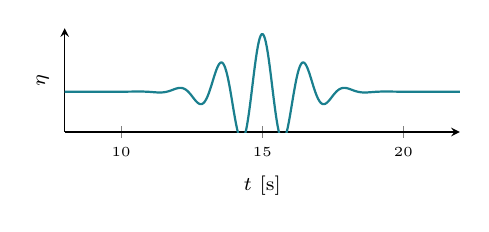
\begin{tikzpicture}
      \begin{axis}[width=6.6cm, height=2.9cm, axis lines=left, xlabel={\scriptsize $t$ [s]},
        ylabel={\scriptsize $\eta$}, ticklabel style={font=\tiny}, ytick=\empty,
        xmin=8, xmax=22, ymin=-0.7, ymax=1.1, samples=400, domain=8:22]
        \addplot[sea, thick] {exp(-((x-15)^2)/3.2)*cos(deg(2*pi*(x-15)/1.5))};
      \end{axis}
    \end{tikzpicture}
  \end{columns}
\end{frame}

% ----------------------------------------------------------------------
\begin{frame}[fragile]{The \texttt{relaxationZone} block and the outlet}
  \begin{columns}[T]
    \column{0.44\textwidth}
\begin{lstlisting}[language=foam]
relaxationZone
{
    relaxationScheme Spatial;
    relaxationShape  Rectangular;
    beachType        Empty;

    relaxType   INLET;      // or OUTLET
    startX      (0 0 -1);   // box corner
    endX        (3 0  1);   // box corner
    orientation (1 0 0);    // points into
}                           // the domain
\end{lstlisting}
\begin{lstlisting}[language=foam]
outletCoeffs
{
    waveType  potentialCurrent;
    U         (0 0 0);      // target: rest
    Tsoft     2;
    relaxationZone { relaxType OUTLET;
        startX (12 0 -1); endX (18 0 1); ... }
};
\end{lstlisting}
    \column{0.53\textwidth}\small
    \renewcommand{\arraystretch}{1.15}
    \begin{tabularx}{\linewidth}{@{}P{2.6cm}L@{}}
      \toprule
      \key{relaxationScheme} & \key{Spatial}: weight depends on position in the zone \\
      \key{relaxationShape}  & \key{Rectangular}: a box from \key{startX} to \key{endX} (also \key{Semicylindrical}, \key{Frozen}) \\
      \key{beachType}        & \key{Empty}: no extra numerical beach \\
      \key{relaxType}        & \key{INLET}: weight 0 at the start of the box (pure target) and 1 at its inner edge.
                               \key{OUTLET} flips the direction \\
      \key{orientation}      & direction from the boundary into the domain \\
      \bottomrule
    \end{tabularx}

    \vspace{1mm}
    \textbf{Outlet}: the target is still water (\key{potentialCurrent} with $\mathbf{U}=0$). The zone
    removes the wave gradually over 6 m ($\approx 2L$), so little is reflected.
  \end{columns}
\end{frame}

% ----------------------------------------------------------------------
\begin{frame}{Relaxation zone theory}
  \begin{columns}[T]
    \column{0.5\textwidth}\small
    In each zone, after every time step, the computed fields are blended with the target
    (the wave theory, still water, or later the HOS solution):
    \vspace{-2mm}\[
      \boxed{\;\phi \leftarrow w\,\phi_{\text{computed}} + (1-w)\,\phi_{\text{target}}\;}
      \qquad \phi \in \{\mathbf{U}, \alpha\}
    \]
    Exponential weight (Jacobsen et al.\ 2012):
    \[
      w(\sigma) = 1 - \frac{\exp(\sigma^{p}) - 1}{\exp(1) - 1},\qquad p = 3.5
    \]
    $\sigma=0$ at the inner edge (CFD side), $\sigma=1$ at the boundary.
    \begin{itemize}
      \item Smooth $w$: the change is gradual, so the zone itself reflects little
      \item Zone length $\gtrsim$ 1 wavelength (inlet), $\gtrsim$ 2 (outlet)
      \item Reflected waves reaching the inlet zone are absorbed too
    \end{itemize}
    \column{0.47\textwidth}
    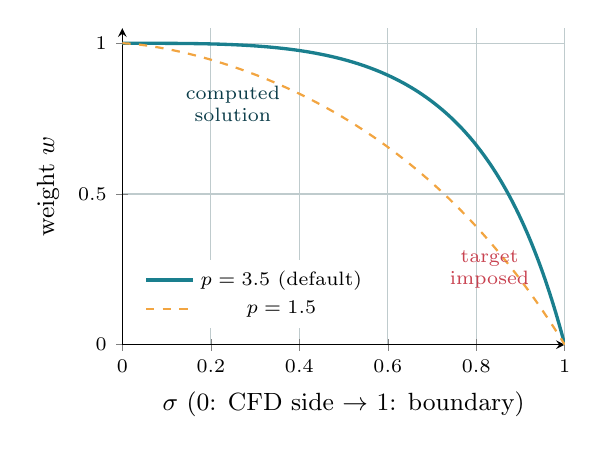
\begin{tikzpicture}
      \begin{axis}[width=7.2cm, height=5.6cm, axis lines=left,
        xlabel={\small $\sigma$ (0: CFD side $\rightarrow$ 1: boundary)},
        ylabel={\small weight $w$}, ticklabel style={font=\scriptsize},
        xmin=0, xmax=1, ymin=0, ymax=1.05, grid=major, grid style={foam!70!mute},
        samples=200, domain=0:1, legend style={font=\scriptsize, draw=none, at={(0.03,0.05)}, anchor=south west}]
        \addplot[sea, very thick] {1 - (exp(x^3.5)-1)/(exp(1)-1)};
        \addlegendentry{$p=3.5$ (default)}
        \addplot[sand, thick, dashed] {1 - (exp(x^1.5)-1)/(exp(1)-1)};
        \addlegendentry{$p=1.5$}
        \node[font=\scriptsize, deep, align=center] at (axis cs:0.25,0.8) {computed\\solution};
        \node[font=\scriptsize, coral, align=center] at (axis cs:0.83,0.25) {target\\imposed};
      \end{axis}
    \end{tikzpicture}
  \end{columns}
\end{frame}

% ----------------------------------------------------------------------
\begin{frame}[fragile]{The mesh: \texttt{system/blockMeshDict}}
  \begin{columns}[T]
    \column{0.42\textwidth}
\begin{lstlisting}[language=foam]
x0 0;  x1 18;           // length
y0 -0.01; y1 0.01;      // 1 cell (2D)
z0 -0.5; z1 -0.15;      // bottom layer
z2  0.15; z3 0.3;       // band, air

nx  720;   // dx = 0.025
nz0  10;   // dz = 0.035  bottom
nz1  30;   // dz = 0.010  surface band
nz2   6;   // dz = 0.025  air
\end{lstlisting}
    \small
    \begin{itemize}
      \item Three stacked blocks, uniform inside
      \item Patches: \key{inlet}, \key{outlet}, \key{bottom} (wall), \key{atmosphere}, \key{frontBack} (empty)
    \end{itemize}
    \column{0.55\textwidth}
    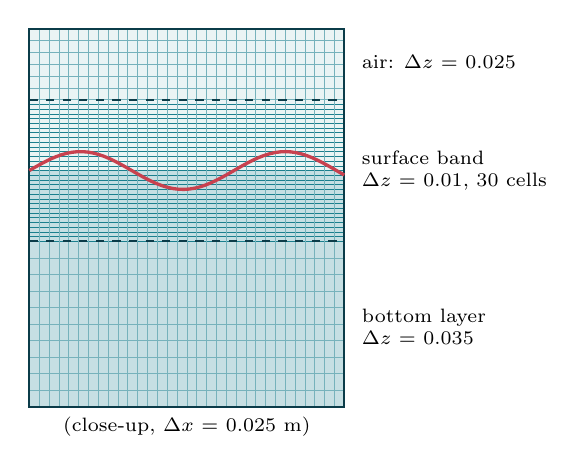
\begin{tikzpicture}[x=1cm,y=6cm]
      % bands
      \fill[sea!25] (0,-0.5) rectangle (4,0);
      \fill[foam] (0,0) rectangle (4,0.3);
      \foreach \z in {-0.5,-0.465,...,-0.15} \draw[sea!60, line width=0.2pt] (0,\z) -- (4,\z);
      \foreach \z in {-0.15,-0.14,...,0.15} \draw[sea, line width=0.2pt] (0,\z) -- (4,\z);
      \foreach \z in {0.15,0.175,...,0.3} \draw[sea!60, line width=0.2pt] (0,\z) -- (4,\z);
      \foreach \x in {0,0.125,...,4} \draw[sea!60, line width=0.2pt] (\x,-0.5) -- (\x,0.3);
      \draw[deep, thick] (0,-0.5) rectangle (4,0.3);
      \draw[coral, very thick, domain=0:4, samples=60] plot (\x,{0.04*sin(deg(2*pi*\x/2.6))});
      \draw[deep, thick, dashed] (0,-0.15) -- (4,-0.15); \draw[deep, thick, dashed] (0,0.15) -- (4,0.15);
      \node[right, font=\scriptsize, align=left] at (4.1,0.23) {air: $\Delta z$ = 0.025};
      \node[right, font=\scriptsize, align=left] at (4.1,0) {surface band\\$\Delta z$ = 0.01, 30 cells};
      \node[right, font=\scriptsize, align=left] at (4.1,-0.33) {bottom layer\\$\Delta z$ = 0.035};
      \node[below, font=\scriptsize] at (2,-0.5) {(close-up, $\Delta x$ = 0.025 m)};
    \end{tikzpicture}

    \vspace{1mm}
    \begin{tabular}{ccc}
      {\color{sea}\LARGE\bfseries 33\,120} & {\color{sea}\LARGE\bfseries 113} & {\color{sea}\LARGE\bfseries 8}\\
      \scriptsize cells & \scriptsize cells per $L$ & \scriptsize cells per $H$
    \end{tabular}
  \end{columns}

  \vspace{1mm}
  \small\textbf{Why:} the band $|z|<0.15$ m holds the whole wave ($\pm H/2$ plus margin) at fine $\Delta z$. Below
  and above, the flow is smooth and coarser cells suffice. Rule of thumb: $\gtrsim$ 100 cells per $L$, $\gtrsim$ 8--10 per $H$.
\end{frame}

% ----------------------------------------------------------------------
\begin{frame}[fragile]{Surface elevation gauges}
  \begin{columns}[T]
    \column{0.5\textwidth}
    \small\file{constant/probeDefinitions}
\begin{lstlisting}[language=foam]
surfaceElevation
{
    type              waveGauge;
    pointDistribution userDefinedDistribution;
    N        6;
    xValues  nonuniform 6(2 4 6 8 10 12);
    yValues  uniform 0;
    zValues  uniform -0.49;   // line start
    add      (0 0 0.78);      // line vector
    axis     z;
    writeControl  adjustableRunTime;
    writeInterval 0.02;       // 50 Hz
}
\end{lstlisting}
    \small
    \texttt{waveGaugesNProbes} turns this into a function object that \file{controlDict} includes.
    \column{0.47\textwidth}\small
    \textbf{How a gauge measures $\eta$}: sample $\alpha$ along a vertical line from $z_0$ and integrate
    \[
      \eta = z_0 + \int_{z_0}^{z_0+\ell} \alpha\,dz
      \approx z_0 + \sum_i \tfrac12(\alpha_i+\alpha_{i+1})\,\Delta z_i
    \]
    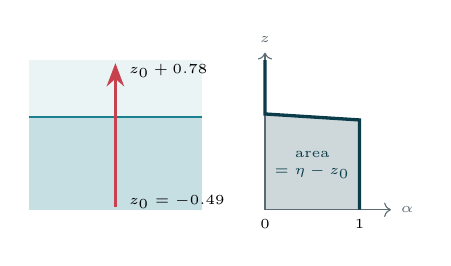
\begin{tikzpicture}[x=1cm,y=1.9cm]
      \fill[sea!25] (0,0) rectangle (2.2,0.62);
      \fill[foam] (0,0.62) rectangle (2.2,1);
      \draw[sea, thick] (0,0.62) -- (2.2,0.62);
      \draw[coral, very thick, -{Stealth}] (1.1,0.02) -- (1.1,0.98);
      \node[font=\tiny, right] at (1.15,0.05) {$z_0=-0.49$};
      \node[font=\tiny, right] at (1.15,0.93) {$z_0+0.78$};
      \fill[deep!20] (3,0) -- (4.2,0) -- (4.2,0.6) -- (3,0.64) -- cycle;
      \draw[mute,->] (3,0) -- (4.6,0) node[right, font=\tiny] {$\alpha$};
      \draw[mute,->] (3,0) -- (3,1.05) node[above, font=\tiny] {$z$};
      \draw[deep, very thick] (4.2,0) -- (4.2,0.6) -- (3,0.64) -- (3,1);
      \node[font=\tiny, below] at (4.2,0) {1};
      \node[font=\tiny, below] at (3,0) {0};
      \node[font=\tiny, deep, align=center] at (3.6,0.3) {area\\$=\eta-z_0$};
    \end{tikzpicture}

    \textbf{Output}: \file{postProcessing/surfaceElevation/\\0/surfaceElevation.dat}
    \begin{itemize}
      \item header rows \texttt{-1}, \texttt{-2}, \texttt{-3}: $x$, $y$, $z$ of each gauge
      \item then one row per time: $t$, $\eta_1$, \dots, $\eta_6$
    \end{itemize}
  \end{columns}
\end{frame}

% ----------------------------------------------------------------------
\begin{frame}{Boundary conditions (\texttt{0.orig})}
  \footnotesize
  \renewcommand{\arraystretch}{1.15}
  \begin{tabularx}{\linewidth}{@{}P{1.8cm}P{2.1cm}P{2.3cm}P{3.0cm}L@{}}
    \toprule
    Patch & \key{alpha.water} & \key{U} & \key{p\_rgh} & Meaning \\
    \midrule
    \key{inlet}  & zeroGradient & zeroGradient & fixedFluxExtrapolated & The \emph{zone} makes the wave. The boundary is in the zone where $w = 0$, so the target is imposed next to it \\
    \key{outlet} & zeroGradient & zeroGradient & fixedFluxExtrapolated & Same: the outlet zone has already damped the wave \\
    \key{bottom} & zeroGradient & slip & fixedFluxExtrapolated & Impermeable, frictionless floor (no boundary layer to resolve) \\
    \key{atmosphere} & inletOutlet (0) & pressureInlet\-Outlet\-Velocity & totalPressure $p_0=0$ & Open top: air flows in and out freely. Air (not water) enters on inflow \\
    \key{frontBack} & empty & empty & empty & 2D \\
    \bottomrule
  \end{tabularx}

  \vspace{2mm}\small
  \begin{itemize}
    \item \textbf{fixedFluxExtrapolatedPressure}: sets the pressure gradient so that it matches the
          boundary flux (the multiphase version of fixedFluxPressure). Correct with gravity and density jumps
    \item \key{p\_rgh} $= p - \rho\,\mathbf{g}\cdot\mathbf{x}$: hydrostatics are taken out, so the top can be $p_0=0$
  \end{itemize}
\end{frame}

% ----------------------------------------------------------------------
\begin{frame}{Discretisation schemes (\texttt{system/fvSchemes})}
  \footnotesize
  \renewcommand{\arraystretch}{1.1}
  \begin{tabularx}{\linewidth}{@{}P{3.0cm}P{4.6cm}L@{}}
    \toprule
    Term & Scheme & Why \\
    \midrule
    \key{ddt} & \key{Euler} & Implicit, bounded, robust. With Co $\le 0.5$ the time error is small \\
    \key{div(rhoPhi,U)} & \key{Gauss limitedLinearV 1} & Second order, TVD-limited. ``V'' limits along the direction of steepest change, so no wiggles at the density jump \\
    \key{div(phi,alpha)} & \key{Gauss vanLeer01} & MULES (waveFoam): bounded $0\le\alpha\le1$ \\
    \key{div(phirb,alpha)} & \key{Gauss interfaceCompression} & MULES: keeps the interface sharp (\key{cAlpha 1}). waveIsoFoam does not use either: isoAdvector advects $\alpha$ geometrically \\
    \key{grad} & \key{Gauss linear} & Second order, mesh is orthogonal hex \\
    \key{laplacian} & \key{Gauss linear limited corrected 0.5} & Non-orthogonal correction, limited for safety \\
    \key{interpolation} / \key{snGrad} & \key{linear} / \key{corrected} & Standard second order \\
    \key{fluxRequired} & \key{p\_rgh}, \key{pcorr}, \key{alpha.water} & Fluxes needed by the pressure correction and the $\alpha$ advection \\
    \key{ddtCorr} & \key{on} & FoamWaveTank switch: keep the ddtCorr flux correction in the pressure equation \\
    \bottomrule
  \end{tabularx}
\end{frame}

% ----------------------------------------------------------------------
\begin{frame}[fragile]{Solution and time control}
  \begin{columns}[T]
    \column{0.52\textwidth}\small
    \textbf{\file{fvSolution}}
    \begin{itemize}
      \item \key{PIMPLE}: \key{nOuterCorrectors 1} (PISO mode), \key{nCorrectors 3},
            \key{momentumPredictor yes}, \key{nNonOrthogonalCorrectors 1}
      \item \key{p\_rgh}: GAMG, tol $10^{-5}$. \key{U}: PBiCGStab + DILU
      \item isoAdvector (waveIsoFoam): \key{reconstructionScheme plicRDF},
            \key{isoFaceTol 1e-6}, \key{surfCellTol 1e-3}, \key{nAlphaBounds 3}, \key{clip true}
      \item MULES (waveFoam): \key{nAlphaCorr 3}, \key{nLimiterIter 5}, \key{cAlpha 1}
      \item Laminar (\file{turbulenceProperties}): non-breaking waves; RANS models damp waves artificially
    \end{itemize}
    \column{0.45\textwidth}\small
    \textbf{\file{controlDict}}
\begin{lstlisting}[language=foam]
application     waveIsoFoam;
endTime         20;
adjustTimeStep  yes;
maxCo           0.5;   // momentum
maxAlphaCo      0.5;   // interface
maxDeltaT       0.05;
writeInterval   0.5;
libs ( "libwaves2Foam.so" );
functions
{ #includeIfPresent "../waveGaugesNProbes/
      surfaceElevation_controlDict"; }
\end{lstlisting}
    \textbf{Why Co $\le$ 0.5}: phase and amplitude errors grow with Co. The wave travels
    $\sim$\,$L/T$, and too large a step damps it along the tank.
  \end{columns}
\end{frame}

% ----------------------------------------------------------------------
\begin{frame}[fragile]{waveFoam vs.\ waveIsoFoam: measure the damping}
  \begin{columns}[T]
    \column{0.5\textwidth}\small
    The same three cases in two folders. Only \key{application} differs:
    \begin{itemize}
      \item \textbf{waveFoam}: algebraic VOF (MULES + interface compression)
      \item \textbf{waveIsoFoam}: geometric VOF (isoAdvector, PLIC), sharper interface
    \end{itemize}
    Both use the same waves2Foam relaxation zones.

    \vspace{2mm}
    \textbf{Question}: how much wave height does each lose between $x=4$ and $x=12$ m?
    \column{0.47\textwidth}
\begin{lstlisting}[style=sh]
cd Day1_Waves/HandsonExercise
(cd waveIsoFoam/01_regularWaves && ./Allrun)
(cd waveFoam/01_regularWaves    && ./Allrun)

# from Day1_Waves/HandsonExercise
python3 ../../Tools/waveStats.py \
    waveFoam/01_regularWaves \
    waveIsoFoam/01_regularWaves \
    --start 12
\end{lstlisting}
    \small \texttt{waveStats.py}: mean wave height, crest, trough and period at every gauge, for CFD
    or HOS-NWT cases. Options \texttt{--start}, \texttt{--end}.
  \end{columns}
\end{frame}

% ======================================================================
\sectionframe{Part 2}{HOS-NWT: potential-flow waves}

% ----------------------------------------------------------------------
\begin{frame}{What is HOS?}
  \begin{columns}[T]
    \column{0.55\textwidth}\small
    \textbf{High-Order Spectral method}: nonlinear potential flow (inviscid,
    irrotational), $\nabla^2\phi = 0$, solved only on the free surface.

    Unknowns: $\eta(x,t)$ and the surface potential $\tilde\phi(x,t)=\phi(x,\eta,t)$.
    Zakharov form of the free-surface conditions:
    \begin{align*}
      \frac{\partial\eta}{\partial t} &= (1+|\nabla\eta|^2)\,W - \nabla\tilde\phi\cdot\nabla\eta\\
      \frac{\partial\tilde\phi}{\partial t} &= -g\eta - \tfrac12|\nabla\tilde\phi|^2 + \tfrac12(1+|\nabla\eta|^2)\,W^2
    \end{align*}
    $W$ = vertical velocity at the surface, from a series expansion of $\phi$ up to
    order $M$ (\textbf{HOS nonlinearity order}, here 3).

    In the closed tank (HOS-NWT), $\phi$ is a sum of modes
    \[
      \phi = \sum_n A_n(t)\cos(k_n x)\frac{\cosh k_n(z+h)}{\cosh k_n h} + \phi_{\text{wavemaker}},
      \quad k_n=\frac{n\pi}{L}
    \]
    \column{0.42\textwidth}\small
    \textbf{Why use it}
    \begin{itemize}
      \item FFT-based: very fast, 2D or 3D, long tanks and durations
      \item Accurate nonlinear propagation (dispersion, focusing)
      \item Wavemaker like the lab: piston or flap
    \end{itemize}
    \textbf{Limits}
    \begin{itemize}
      \item No breaking, no viscosity, no bodies
      \item Very steep waves stop the run (time step collapses): use filtering
    \end{itemize}
    \textbf{So}: HOS for the wave, CFD only where the physics needs it, around the body.

    \vspace{1mm}
    \scriptsize Ducrozet et al.\ (2012), HOS-NWT: \url{https://gitlab.com/lheea/HOS-NWT}
  \end{columns}
\end{frame}

% ----------------------------------------------------------------------
\begin{frame}[fragile]{HOS-NWT input: \texttt{HOS/RegularWaves/input\_HOS-NWT.yml}}
  \begin{columns}[T]
    \column{0.52\textwidth}
\begin{lstlisting}[language=bash]
wave tank:
  dimensions: {length: 20., depth: 0.5}
  wavemaker:  {type: piston}
  numerical absorption beach:
    position ratio: 0.75       # beach from 15 m
    absorption coefficient: 1.
computation case:
  3D: false
  type: regular
  amplitude: 0.04              # m (H = 0.08)
  frequency: 0.666667          # Hz (T = 1.5 s)
time:
  duration: 32.0               # >= refTime + CFD endTime
  ramping: {order: 2, duration: 3.}
numerical parameters:
  time integration tolerance: 1.e-5
  discretization: {x: 512, z: 17}  # modes
  HOS nonlinearity order: 3
  wavemaker nonlinearity order: 2
  dealiasing: {x: 3}
output:
  directory: Results
  frequency: 20.               # Hz, modes file too
  volumic modal data: standard # -> modes_HOS_SWENSE.dat
  probes: {type: free surface elevation,
           position file: prob.inp}
\end{lstlisting}
    \column{0.45\textwidth}\small
    \begin{itemize}
      \item \textbf{wave tank}: length, depth, wavemaker, beach (last 25\%)
      \item \textbf{computation case}: what wave to make (next slide)
      \item \textbf{duration}: must cover the CFD window, \key{referenceTime} + CFD \key{endTime}
      \item \textbf{discretization x}: 512 modes, $\Delta x$ = 0.039 m;
            \textbf{z}: modes on the wavemaker
      \item \textbf{order 3}: nonlinear terms up to 3rd order
      \item \textbf{output frequency}: also the time resolution Grid2Grid interpolates
      \item \textbf{volumic modal data}: writes the modes file for the coupling
      \item \file{prob.inp}: one $x$ per line, here 7 \dots 11 m
    \end{itemize}
    \scriptsize (YAML shown compacted; the case file has one key per line.)
  \end{columns}
\end{frame}

% ----------------------------------------------------------------------
\begin{frame}[fragile]{Wave types and wavemakers in HOS-NWT}
  \begin{columns}[T]
    \column{0.31\textwidth}
    {\small\bfseries\color{deep} Regular}
\begin{lstlisting}[language=bash]
type: regular
amplitude: 0.04   # m
frequency: 0.666667
\end{lstlisting}
    \scriptsize Linear wavemaker transfer. The nonlinear wave can come out higher than $2a$:
    \texttt{MooredBoxRegularWaves} needs $a$ = 0.0576 m for $H$ = 0.1195 m.
    \column{0.31\textwidth}
    {\small\bfseries\color{deep} Irregular}
\begin{lstlisting}[language=bash]
type: analytical spectrum
spectrum: JONSWAP
Hs: 0.06
Tp: 1.5
gamma: 3.3
seed: 1000
\end{lstlisting}
    \scriptsize Change \texttt{seed} for another realisation of the same sea state.
    \column{0.33\textwidth}
    {\small\bfseries\color{deep} Focused: from a file}
\begin{lstlisting}[language=bash]
type: file
format: cfg+dat
file: focusedWave
\end{lstlisting}
    \scriptsize \file{focusedWave.cfg} + \file{.dat}: amplitude and phase per frequency, written by
\begin{lstlisting}[style=sh]
python3 Tools/makeFocusedWaveHOS.py \
   --A 0.06 --Tp 1.5 \
   --xf 9 --tf 25
\end{lstlisting}
  \end{columns}

  \vspace{4mm}
  \begin{columns}[T]
    \column{0.5\textwidth}
    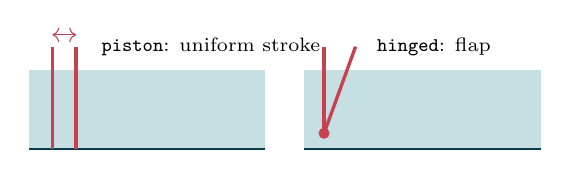
\begin{tikzpicture}[x=0.5cm,y=0.5cm]
      \fill[sea!25] (0,0) rectangle (6,2);
      \draw[deep, thick] (0,0) -- (6,0);
      \draw[coral, very thick] (0.6,0) -- (0.6,2.6); \draw[coral, very thick] (1.2,0) -- (1.2,2.6);
      \draw[coral, <->] (0.6,2.9) -- (1.2,2.9);
      \node[font=\scriptsize, right] at (1.6,2.6) {\texttt{piston}: uniform stroke};
      \fill[sea!25] (7,0) rectangle (13,2);
      \draw[deep, thick] (7,0) -- (13,0);
      \draw[coral, very thick] (7.5,0.4) -- (7.5,2.6); \draw[coral, very thick] (7.5,0.4) -- (8.3,2.6);
      \fill[coral] (7.5,0.4) circle (2pt);
      \node[font=\scriptsize, right] at (8.6,2.6) {\texttt{hinged}: flap};
    \end{tikzpicture}
    \column{0.47\textwidth}\small
    \texttt{WavemakerMotion/\{Piston,Flap\}}: the same wave from both. Compare
    \file{Results/wmk\_motion.dat}. A flap gives deep-water-like velocity profiles.
  \end{columns}
\end{frame}

% ----------------------------------------------------------------------
\begin{frame}[fragile]{Running HOS-NWT and what comes out}
  \begin{columns}[T]
    \column{0.5\textwidth}
\begin{lstlisting}[style=sh]
cd potentialFlowWaves/HOS/RegularWaves
./Allrun        # HOS-NWT on the PATH, or:
HOSNWT=/path/to/HOS-NWT ./Allrun

# start again
./Allclean && ./Allrun

# wave statistics at the HOS probes
python3 ../../../../../Tools/waveStats.py .
\end{lstlisting}
    \small
    \textbf{Allrun checks completion}: HOS-NWT exits with code 0 even when the time step
    collapses (``minimum time step reached''). \texttt{Allrun} compares the last time in
    \file{vol\_energy.dat} with \texttt{duration}.
    \column{0.47\textwidth}\small
    \renewcommand{\arraystretch}{1.2}
    \begin{tabularx}{\linewidth}{@{}P{3.3cm}L@{}}
      \toprule
      \file{Results/...} & Content \\
      \midrule
      \file{probes.dat} & $\eta(t)$ at the \file{prob.inp} positions \\
      \file{modes\_HOS\_SWENSE.dat} & modal amplitudes in time, \textbf{read by Grid2Grid} \\
      \file{wmk\_motion.dat} & wavemaker stroke \\
      \file{vol\_energy.dat} & volume and energy in time (conservation check) \\
      \file{log.HOS-NWT} & screen output (in the case folder) \\
      \bottomrule
    \end{tabularx}

    \vspace{2mm}
    \textbf{Run stops early?} Lower the steepness, or add \texttt{filtering coefficients: x: 0.6}
    (as in \texttt{WavemakerMotion} and the floating-box cases).
  \end{columns}
\end{frame}

% ======================================================================
\sectionframe{Part 3}{Coupling HOS and OpenFOAM with Grid2Grid}

% ----------------------------------------------------------------------
\begin{frame}{The idea: HOS brings the wave, CFD resolves the details}
  \centering
  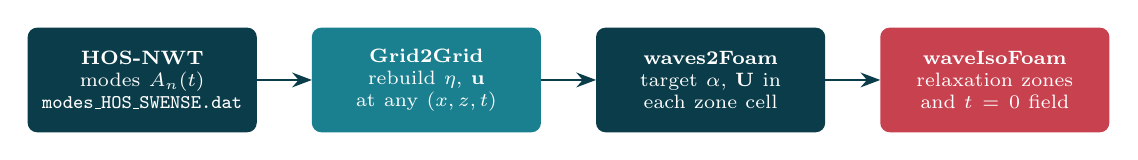
\begin{tikzpicture}[node distance=7mm]
    \node[dbox, text width=2.6cm, minimum height=1.3cm] (h) {HOS-NWT\\{\normalfont modes $A_n(t)$}\\\file{\color{white}modes\_HOS\_SWENSE.dat}};
    \node[dbox, text width=2.6cm, minimum height=1.3cm, right=of h, fill=sea, draw=sea] (g) {Grid2Grid\\{\normalfont rebuild $\eta$, $\mathbf{u}$ at any $(x,z,t)$}};
    \node[dbox, text width=2.6cm, minimum height=1.3cm, right=of g] (w) {waves2Foam\\{\normalfont target $\alpha$, $\mathbf{U}$ in each zone cell}};
    \node[dbox, text width=2.6cm, minimum height=1.3cm, right=of w, fill=coral, draw=coral] (c) {waveIsoFoam\\{\normalfont relaxation zones and $t=0$ field}};
    \draw[arr] (h) -- (g); \draw[arr] (g) -- (w); \draw[arr] (w) -- (c);
  \end{tikzpicture}

  \vspace{5mm}
  \begin{columns}[T]
    \column{0.48\textwidth}\small
    \textbf{Grid2Grid} (LHEEA, Centrale Nantes)
    \begin{itemize}
      \item Reads the HOS modal file
      \item Evaluates the modes on its own grid: $x$ from HOS, $z$ from \file{Grid2Grid.dict}
      \item Interpolates in space and time (order 3 = cubic splines), so any CFD cell
            centre and time step can be served
      \item Linked into waves2Foam: \key{externalForcing Grid2Grid}
    \end{itemize}
    \column{0.48\textwidth}\small
    \textbf{In the CFD}
    \begin{itemize}
      \item The HOS solution is the \emph{target} of both relaxation zones
      \item \texttt{setWaveField} uses it as the initial field, so the CFD starts with
            waves already in the domain
      \item The CFD domain can be short: only the region of interest
    \end{itemize}
  \end{columns}
\end{frame}

% ----------------------------------------------------------------------
\begin{frame}{Geometry and the space-time mapping}
  \centering
  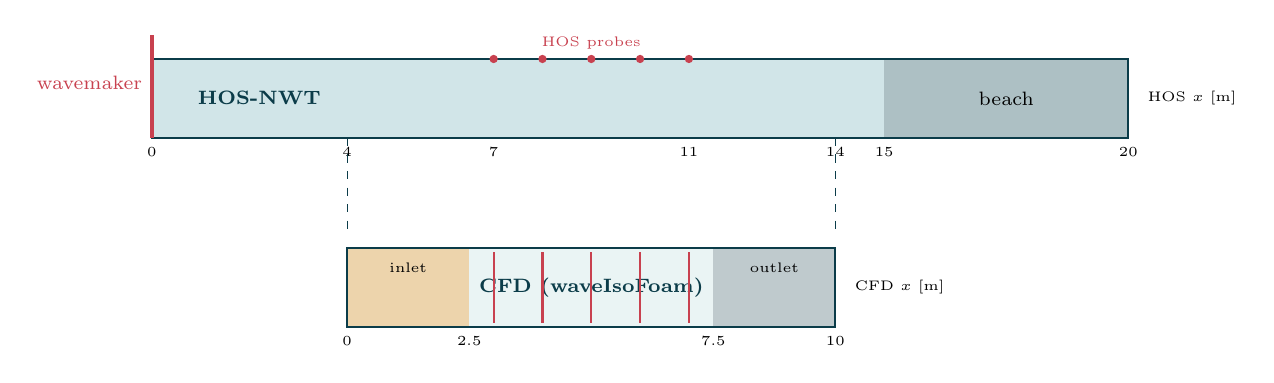
\begin{tikzpicture}[x=0.62cm, y=1cm]
    % HOS tank
    \fill[sea!20] (0,0) rectangle (20,1);
    \fill[mute, opacity=0.3] (15,0) rectangle (20,1);
    \draw[deep, thick] (0,0) rectangle (20,1);
    \draw[coral, ultra thick] (0,0) -- (0,1.3);
    \node[font=\scriptsize, left, coral] at (0,0.7) {wavemaker};
    \node[font=\scriptsize\bfseries, deep] at (2.2,0.5) {HOS-NWT};
    \node[font=\scriptsize] at (17.5,0.5) {beach};
    \foreach \x in {0,4,7,11,14,15,20} \node[font=\tiny, below] at (\x,0) {\x};
    \foreach \x in {7,8,9,10,11} \fill[coral] (\x,1) circle (1.5pt);
    \node[font=\tiny, coral, above] at (9,1) {HOS probes};
    % CFD window
    \draw[deep, dashed] (4,0) -- (4,-1.2); \draw[deep, dashed] (14,0) -- (14,-1.2);
    \fill[foam] (4,-2.4) rectangle (14,-1.4);
    \fill[sand, opacity=0.4] (4,-2.4) rectangle (6.5,-1.4);
    \fill[mute, opacity=0.3] (11.5,-2.4) rectangle (14,-1.4);
    \draw[deep, thick] (4,-2.4) rectangle (14,-1.4);
    \node[font=\scriptsize\bfseries, deep] at (9,-1.9) {CFD (waveIsoFoam)};
    \node[font=\tiny] at (5.25,-1.65) {inlet};
    \node[font=\tiny] at (12.75,-1.65) {outlet};
    \foreach \x/\l in {4/0,6.5/2.5,11.5/7.5,14/10} \node[font=\tiny, below] at (\x,-2.4) {\l};
    \foreach \x in {7,8,9,10,11} \draw[coral, thick] (\x,-2.35) -- (\x,-1.45);
    \node[font=\tiny, right] at (14.2,-1.9) {CFD $x$ [m]};
    \node[font=\tiny, right] at (20.2,0.5) {HOS $x$ [m]};
  \end{tikzpicture}

  \vspace{4mm}
  \begin{columns}[T]
    \column{0.48\textwidth}
    \[
      \boxed{x_{\text{HOS}} = x_{\text{CFD}} - \texttt{referencePosition}}
    \]
    \small \key{referencePosition (-4 0 0)}: CFD $x=0$ is HOS $x=4$ m. The CFD gauges
    3 \dots 7 m sit on the HOS probes 7 \dots 11 m.
    \column{0.48\textwidth}
    \[
      \boxed{t_{\text{HOS}} = t_{\text{CFD}} + \texttt{referenceTime}}
    \]
    \small \key{referenceTime 10}: CFD $t=0$ is HOS $t=10$ s, when the wave has filled
    the window. So HOS \texttt{duration} $\ge$ 10 + CFD \key{endTime}.
  \end{columns}
\end{frame}

% ----------------------------------------------------------------------
\begin{frame}[fragile]{\texttt{constant/Grid2Grid.dict}}
  \begin{columns}[T]
    \column{0.46\textwidth}
\begin{lstlisting}[language=foam]
Grid2Grid       HOSNWT;   // which sub-dict

HOSNWT
{
    type                NWT;
    fileType            ASCII;
    filePath            ../../HOS/RegularWaves/
                        Results/modes_HOS_SWENSE.dat;
    interpolationOrder  3;

    zMeshType           meshRatio;
    zMin                -0.5;
    zMax                 0.3;
    nZMin               50;
    nZMax               30;
    zMinRatio           3;
    zMaxRatio           3;
}
\end{lstlisting}
    \small\textbf{Modes file in \file{constant/}?} Copy it and point \key{filePath} there:
\begin{lstlisting}[style=sh]
cp ../../HOS/RegularWaves/Results/\
   modes_HOS_SWENSE.dat constant/
# Grid2Grid.dict:
#   filePath constant/modes_HOS_SWENSE.dat;
\end{lstlisting}
    \column{0.51\textwidth}\scriptsize
    \renewcommand{\arraystretch}{1.12}
    \begin{tabularx}{\linewidth}{@{}P{3.1cm}L@{}}
      \toprule
      \key{Grid2Grid} & name of the sub-dictionary to use \\
      \key{type} & \key{NWT} = HOS-NWT (tank with wavemaker); \key{Ocean} = HOS-Ocean (periodic) \\
      \key{fileType} & format of the modes file: \key{ASCII} (or \key{HDF5}) \\
      \key{filePath} & modes file, \textbf{relative to the CFD case} (or absolute) \\
      \key{interpolationOrder} & spline order in space and time: 1 linear, 3 cubic \\
      \key{zMeshType} & vertical grid on which velocities are rebuilt: \key{meshRatio} (fine near $z=0$), \key{uniform}, \dots \\
      \key{zMin}, \key{zMax} & bottom and top of that grid: the CFD domain ($-h$ and top of air) \\
      \key{nZMin}, \key{nZMax} & points below / above $z=0$ \\
      \key{zMinRatio},\newline\key{zMaxRatio} & $\Delta z_{\max}/\Delta z_{\min}$ below / above $z=0$ \\
      \bottomrule
    \end{tabularx}

  \end{columns}
\end{frame}

% ----------------------------------------------------------------------
\begin{frame}[fragile]{\texttt{waveProperties.input} for the coupled case}
  \begin{columns}[T]
    \column{0.5\textwidth}
\begin{lstlisting}[language=foam]
seaLevel            0.0;
relaxationNames     (inlet outlet);
initializationName  inlet;   // t=0 from HOS

externalForcing     Grid2Grid;

Grid2GridCoeffs
{
    waveType                Grid2Grid;
    Grid2GridInputFileName  Grid2Grid.dict;
    referencePosition       (-4 0 0);
    referenceTheta          0;
    referenceTime           10;
    Tsoft                   0;
}

inletCoeffs
{
    waveType                externalSource;
    Grid2GridInputFileName  Grid2Grid.dict;
    Tsoft                   0;
    relaxationZone { relaxType INLET;
        startX (0 0 -1); endX (2.5 0 1); ... }
};
outletCoeffs    // same, OUTLET, x = 7.5 .. 10
\end{lstlisting}
    \column{0.47\textwidth}\small
    \renewcommand{\arraystretch}{1.15}
    \begin{tabularx}{\linewidth}{@{}P{3.2cm}L@{}}
      \toprule
      \key{externalForcing} & use Grid2Grid as wave source \\
      \key{waveType Grid2Grid} & the global forcing (in \key{Grid2GridCoeffs}) \\
      \key{Grid2GridInput-}\newline\key{FileName} & dict in \file{constant/} \\
      \key{referencePosition} & HOS origin in CFD coordinates (sign!) \\
      \key{referenceTheta} & rotation of the HOS axis (3D) \\
      \key{referenceTime} & HOS time at CFD $t=0$ \\
      \key{waveType externalSource} & the zone's target comes from Grid2Grid \\
      \bottomrule
    \end{tabularx}

    \vspace{2mm}
    \alert{\key{Tsoft 0}} everywhere: with a ramp, \texttt{setWaveField} would
    start from still water and the CFD would not begin with the HOS field.
  \end{columns}
\end{frame}

% ----------------------------------------------------------------------
\begin{frame}{Relaxation zones in the coupled tank}
  \centering
  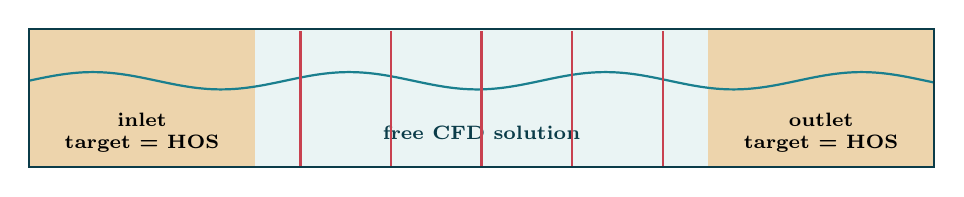
\begin{tikzpicture}[x=1.15cm, y=2.2cm]
    \fill[foam] (0,-0.5) rectangle (10,0.3);
    \fill[sand, opacity=0.4] (0,-0.5) rectangle (2.5,0.3);
    \fill[sand, opacity=0.4] (7.5,-0.5) rectangle (10,0.3);
    \draw[sea, thick, domain=0:10, samples=200] plot (\x,{0.05*sin(deg(2*pi*\x/2.83))});
    \draw[deep, thick] (0,-0.5) rectangle (10,0.3);
    \node[font=\scriptsize\bfseries, align=center] at (1.25,-0.3) {inlet\\target = HOS};
    \node[font=\scriptsize\bfseries, align=center] at (8.75,-0.3) {outlet\\target = HOS};
    \node[font=\scriptsize\bfseries, align=center, deep] at (5,-0.3) {free CFD solution};
    \foreach \x in {3,4,5,6,7} \draw[coral, thick] (\x,-0.49) -- (\x,0.29);
  \end{tikzpicture}

  \vspace{3mm}
  \begin{columns}[T]
    \column{0.48\textwidth}\small
    \textbf{Uncoupled tank} (Part 1)
    \begin{itemize}
      \item Inlet target: wave theory. Outlet target: still water
      \item The outlet must remove the whole wave, so it is long (6 m)
    \end{itemize}
    \column{0.48\textwidth}\small
    \textbf{Coupled tank}
    \begin{itemize}
      \item \emph{Both} zones relax to the HOS wave
      \item The wave leaves on its own. The outlet only removes what the CFD adds:
            reflections, damping and phase errors
      \item So the zones can be short (2.5 m) and the domain small
    \end{itemize}
  \end{columns}
\end{frame}

% ----------------------------------------------------------------------
\begin{frame}[fragile]{Step by step: from HOS to the CFD wave}
  \small
  \begin{columns}[T]
    \column{0.5\textwidth}
    \begin{enumerate}
      \item \textbf{HOS case}: edit \file{input\_HOS-NWT.yml} (wave, duration $\ge$ \key{referenceTime} + \key{endTime})
            and \file{prob.inp}
      \item \textbf{Run HOS}: \texttt{./Allrun}. Check it reached \texttt{duration}
      \item \textbf{Modes file}: \file{Results/modes\_HOS\_SWENSE.dat}. Point
            \key{filePath} in \file{constant/Grid2Grid.dict} to it (or copy it to \file{constant/})
      \item \textbf{Grid2Grid.dict}: \key{zMin}/\key{zMax} = CFD bottom/top
      \item \textbf{waveProperties.input}: \key{externalForcing Grid2Grid},
            \key{referencePosition}, \key{referenceTime}, zones \key{externalSource}, \key{Tsoft 0}
      \item \textbf{probeDefinitions}: CFD gauges on HOS probes ($x_{\text{CFD}} = x_{\text{HOS}} + $ refPos)
    \end{enumerate}
    \column{0.47\textwidth}
    \begin{enumerate}\setcounter{enumi}{6}
      \item \texttt{blockMesh}
      \item \texttt{setWaveParameters}
      \item \texttt{relaxationZoneLayout}
      \item \texttt{setWaveField}: HOS wave at $t=0$. Check it in ParaView
      \item \texttt{waveGaugesNProbes}
      \item \texttt{waveIsoFoam}
      \item \texttt{compareHOS\_CFD.py}
    \end{enumerate}
    \vspace{1mm}
\begin{lstlisting}[style=sh]
cd potentialFlowWaves/CFD/RegularWaves
./Allrun      # steps 2 and 7-12
              # (runs HOS if Results are missing)
\end{lstlisting}
  \end{columns}
\end{frame}

% ----------------------------------------------------------------------
\begin{frame}[fragile]{Comparing HOS and CFD probes}
  \begin{columns}[T]
    \column{0.52\textwidth}
\begin{lstlisting}[style=sh]
# in the CFD case
cd potentialFlowWaves/CFD/RegularWaves
python3 ../../../../../Tools/compareHOS_CFD.py

# or with explicit folders
python3 Tools/compareHOS_CFD.py <CFD-case> \
        --hos <HOS-case> [--no-plot]

# wave statistics, CFD and HOS side by side
python3 Tools/waveStats.py <CFD-case> <HOS-case>
\end{lstlisting}
    \small
    \textbf{What it does}
    \begin{itemize}
      \item reads CFD \file{surfaceElevation.dat} and HOS \file{probes.dat} + \file{prob.inp}
      \item finds the HOS case from \key{filePath} in \file{Grid2Grid.dict}
      \item maps $x$ and $t$ with \key{referencePosition} and \key{referenceTime}
    \end{itemize}
    \column{0.45\textwidth}\small
    \textbf{Output}
    \begin{itemize}
      \item RMS difference per gauge, relative to the HOS wave height
      \item \file{compareHOS\_CFD.png} in the CFD case (with matplotlib)
    \end{itemize}
    \textbf{What to look at}
    \begin{itemize}
      \item Start-up transient in the first periods
      \item Phase shift growing downstream: dispersion error, mesh or time step
      \item Crest height loss along the tank: numerical damping
      \item Example: the steep \texttt{FloatingBoxRegularWaves} needed $\Delta x$ = 0.0125 m and
            Co 0.25 to keep the loss at $\sim$8\%
    \end{itemize}
  \end{columns}
\end{frame}

% ======================================================================
{\setbeamercolor{background canvas}{bg=deep}
 \setbeamertemplate{footline}{}
 \setbeamercolor{normal text}{fg=foam}
 \setbeamercolor{itemize/enumerate body}{fg=foam}
 \setbeamercolor{frametitle}{fg=white}
 \renewcommand{\key}[1]{{\leavevmode\ttfamily\color{sand}#1}}
\begin{frame}[plain]{Hands-on: things to try}
  \small
  \begin{columns}[T]
    \column{0.48\textwidth}\color{foam}
    {\color{sand}\bfseries waves2Foam tank}
    \begin{itemize}
      \item Change $H$ or $T$: watch $H/L$ and the cells per $L$ and per $H$
      \item Halve the outlet zone: does the reflection at $x=12$ grow?
      \item Irregular: $N$ = 50 vs.\ 200, another seed
      \item Focused: move \key{focusPoint} / \key{focusTime}. Is the crest where you asked?
      \item waveFoam vs.\ waveIsoFoam: \texttt{waveStats.py --start 12}
    \end{itemize}
    \column{0.48\textwidth}\color{foam}
    {\color{sand}\bfseries HOS and coupling}
    \begin{itemize}
      \item \texttt{compareHOS\_CFD.py}: phase, crest, start-up transient
      \item Change \key{referenceTime}: start before the wave arrives
      \item \texttt{WavemakerMotion}: piston vs.\ flap stroke and waves
      \item \texttt{makeFocusedWaveHOS.py --xf --tf --A}: new focus
      \item Steeper waves: when does HOS stop? Try \texttt{filtering x: 0.8}
      \item Cases 04--06: the waves of Days 2--4 in the empty tank
    \end{itemize}
  \end{columns}
\end{frame}}

\end{document}
